\chapter{Implementation}
\label{chapter:implementation}

The goal of this thesis was to create a program which automatically generates route data of a pool of jobs at various locations. This chapter describes the process of determining the best tools for the development of the program, the implementation progress itself and the final structure of the program.

\section{Technical decisions}

Technical decisions made early on can greatly effect the final results. Choosing the wrong technologies, for instance, can cause severe setbacks, additional work and in the worst cases completely impede progreess.

\subsection{Generating the routing data}
\label{subsection:routingdata}

To create the all-to-all distance matrix necessary for solving the VRP, it is necessary to use a map routing API which computes the distance of the best route between two nodes and estimates the corresponding traveling time. Since there can be a lot of locations for the algorithm, it is necessary to group nearby targets into one to limit the number of queries made to the API. Even if the routes are generated per technician (i.e. it is necessary to only generate the all-to-all cost matrix from all the jobs assigned to the technician at hand), it is still necessary to make thousands of queries to the map routing API.  

The grouping was performed by picking a random node and assigning its coordinates to other nodes within a 3 kilometre radius. This is then repeated for the remaining untouched nodes until no more merges are possible. While better results could be obtained by picking the merger nodes according to some rules, this simple algorithm is effective enough. The inaccuracy caused by the maximum of 3 kilometre disparity between the real location and the one used for the algorithm should not usually cause big differences in travel time, though with natural formations such as rivers or lakes, this is a possibility.

The number of queries to the map routing API was lowered by 30 - 50 \% by this grouping depending on the test data used. In the number of queries, this provided savings ranging from 1300 to 4000 queries. The more locations involved in the total data, the higher that savings percentage was. This result seems reasonable, as the probability of an additional target being located near an existing one increases as the number of targets increases. The total number of queries made ranged from about 2000 to 4500.

I picked MapQuest\cite{mapquest} to be the routing service provider. They provide 15000 queries per month for free, and that number was high enough for the purpose of this thesis. MapQuest supports getting detailed route information, but for the purpose of this project, only the traveling time value between two locations was used. The routing service provider is easy to replace in the final implementation, as the replacement only requires altering the query made to the service and parsing of the response, so there is no lock-in on a single provider. I tested the quality of MapQuest's routing results by comparing them to the results of other similar services, such as Google maps and Bing maps. The variations between the results was minimal to the point where it was safe to assume that all of them provided good results. 

\subsection{Language requirements}

The most important aspect of choosing which language to use depends on the routing algorithm libraries available for the language. 

Because the algorithm is CPU-intensive, the more low-level languages take precedence over the potentially slower high-level languages. This is not a deciding factor, however, as many of the high-level languages are still sufficiently fast enough for this purpose. Likewise, even if a program written in pure C, for example, might perform better, the increased development time and reduced maintainability are more significant significant issues than a slightly reduced performance of a Java program.

Due to the performance-centric nature of the algorithm, it is important that the language chosen can be profiled to see which parts of the algorithm are the most resource-intensive. Though most modern languages fulfill this requirement, it is worthy of mentioning. 


\subsection{Choosing the library to use}

The important criteria for choosing the libraries to use are performance, solution quality and suitability to the parameters specific to this project. Ease of use and the quality of documentation are also signifcant factors, as well as how well the library is being maintained currently.

My main strategy when picking the library to use was to read the API documentation to see if it supported the functionality I need. Since there are so many different variations of the VRP, there are also numerous types of libraries, most of which were specialised for a specific kind of VRP. If a library was aimed for a different purpose it became apparent quickly. Then I examined how well the library has been maintained and how clear the documentation is.

To see if a library was suitable for my requirements, I looked at the API provided by the library and determined if the API supported the functionality I required. If there was no built-in support, I looked how well the library supported writing additional custom constraints to be use in the route generation. I also considered the number and variety of usage examples as one criterion for the decision, as it is a clear indication whether the library supports the various use cases required in the context of this thesis. This method of choosing a library eventually led me to pick a Java-based library Jsprit by Stefan Schr�der\cite{jsprit}. 


\subsection{Jsprit routing library}
To find solutions to VRP, Jsprit employs the ruin and recreate method desribed in section~\ref{subsection:ruinandrecreate}. Java is a language I am very comfortable with, so my personal preference can also be considerd as a deciding factor.

Jsprit supports many different types of VRP. It allows the programmer to define multiple types of vehicles each with different capacities for various types of items. Each vehicle can have an associated fixed and running costs. The fixed cost is applied for simply using the vehicle (this represents, for example, buying the said vehicle) and running costs signify gasoline usage, service costs (averaged over driving distance) and so on. Additionally, the maximum speed and waiting time costs can be specified for vehicles. For each vehicle, the starting and end location of routes can be set. This essentially means that Jsprit is capable of solving complex MDVRPs.

The jobs of routes are called services, and each service is associated with a location and a time cost. Locations can contain time windows. The traveling costs (time and distance) between locations can be set using costs matrix.  

Jsprit limits the computation time by providing a setting for iterations, with each iteration consisting of one phase of ruining and recreation.

If the built in constraints found in jsprit are not enough to satisfy the programmer's need, the library also supports additional constraints using an API provided by the library. Jsprit then uses these constraints during route creation to check whether the newly created route is valid.
  
This initial choice I made turned out to be a good one and there was little reason to explore other options. The performance, ease of use and quality of results turned out to be as good as I hoped for. Currently the library is mostly maintained and updated by a single person with some random developers providing occasional patches. 

Jsprit has built-in xml generator for outputting the solution's route data. It also allows accessing the solution data programmatically, making it possible to more directly use the information for custom outputting or manipulation of the results. Jsprit also produces rough visualisations of the best solution it has found, as can be seen in Figure~\ref{fig:librarysolution}.

\begin{figure}[h]
  \begin{center}
    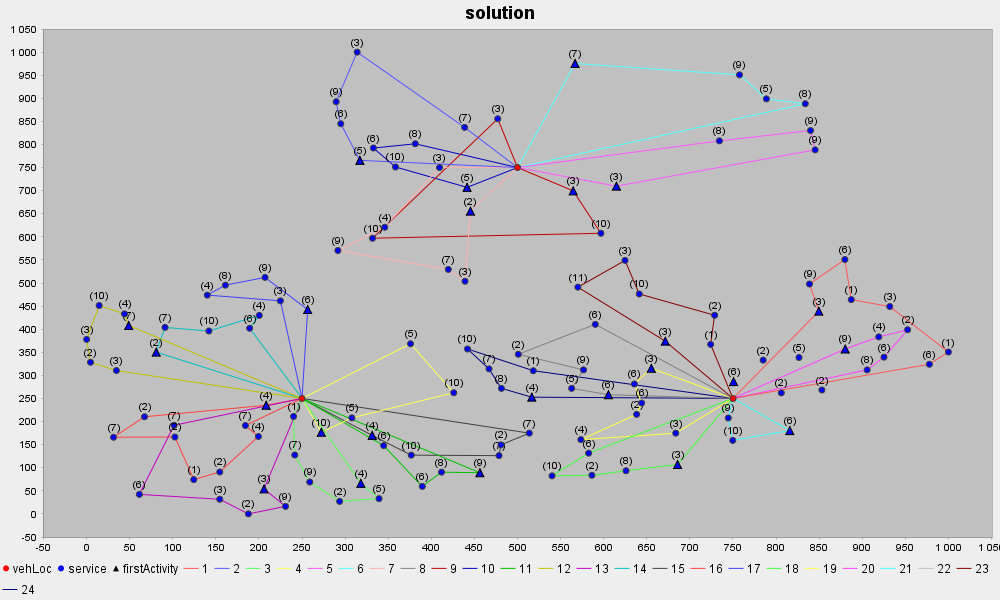
\includegraphics[width=\textwidth]{images/librarysolution.png}
    \caption{An example of the graph output produced by the library. Data unrelated to the business case.}
    \label{fig:librarysolution}
  \end{center}
\end{figure}



\subsection{Other VRP libraries}

I looked into several libraries also made for solving VRPs. This is far from an exhaustive list of the various free libraries available, but might give some pointers for people who are also interested in VRP solving.  

Other libraries I researched were:

\begin{itemize}
\item VRPH: An extensive open source C++ library for solving VRPs. \cite{vrph} 
\item Google's Operations Research tools: A collection of various tools for solving many different types of combinatorial problems. \cite{googleor}
\item Open-VRP: A lisp-based open source library for VRPs. \cite{openvrp}
\item VROOM: A C++-based VRP library. \cite{vroom}
\item OptaPlanner: An open source library capable of solving various combinatorial problems, including VRPs. \cite{optaplanner}
\end{itemize}


\section{Development and structure of the program}

I did the development using the Netbeans IDE. The Jsprit library was the only external library I needed during the development and it was fetched using Maven, a software project management tool.

The development of the program was a straightforward process. I first used some mock data to try out the Jsprit library and see how it performs with some simple fixed problems. Once I was convinced it was functional and expandable piece of software, I proceeded to apply the full business logic, because I had enough experience related to the rest of the project's aspects to know that I would be able to implement them without insurmountable issues. 

To ensure future maintainability, the program was designed to be modular, so if some part of the program needs to changed, the operation will be as easy as possible. The modules of the program are as follows:

\begin{enumerate}  
\item Routing module, transforming address data into a traveling cost matrix. 
\item Job resource demand calculator, abstracting the job resource and man-hour requirements into numbers.
\item The algorithm module, using the traveling cost matrix and job requirements to produce route data.
\item Results visualiser, displaying the results data in a more human-readable form. 
\item Results storing module, converting the results into data suitable to be stored in the client company's database. (not implemented) 
\end{enumerate}

\subsection{Routing module}

The input of this module is the customer data including upcoming jobs and their locations, and the output is a matrix containing the traveling times between these locations. To determine the traveling times, the module makes queries to the map routing API, as demonstrated in subsection~\ref{subsection:routingdata}.

As the many-to-many networks require a lot of queries and a high number of queries leads to higher costs, the module is forced to make some optimisations. Nearby targets are forced into the same location because the difference in traveling times would be minimal. Another benefit of reducing the number of queries is performance. Currently most of the program's time is spent querying the traveling times from the routing API.

When receiving a list of job targets, this module iterates through them and creates new locations if the new target's location is too far from existing ones to be merged to them. Afterwards each target knows the id of the location corresponding with itself. 

With this reduced set of $n$ locations, the module makes $\frac{n^2}{2}$ queries to the routing API. The paths are considered symmetrical, as the traveling time is rarely significantly different depending on which way it is travelled.

All the routing information is cached after fetching it to avoid having to fetch the same data on successive runs if the same input data is used. This also makes consequent uses of the program faster.  

\subsection{Job resource demand calculator}

The estimation as for how long a job will take is currently very coarse. Each installation item takes one hour and each job target has a 15-minute overhead during which contractual business with the customer is done before the work can begin. 

If the job duration added to the back and forth traveling time between the target and the depot is greater than 8.5 hours, the program considers the job too large to complete in one route and splits it. It then calculates the maximum number of installation items that can be handled in one day at the target and creates a new ``subtarget'' which contains the rest of the items. This process is repeated if the new target is again too large to fit on a single day's work schedule. 

For the sake of the algorithm, the subtargets are considered the same as the main targets. However, when outputting solution information, it is important to know which is the main job target item of subtargets.  

\subsection{The algorithm module}

The algorithm module takes the target information and location matrix as input and outputs the solution information ready to be used for whatever purpose. 

Using Jsprit's API, the technician's home is set as the depot and the job targets as the nodes to be visited. The traveling costs matrix is then given to Jsprit. Because Jsprit does not natively support having a maximum route time constraint, I created one using its custom constraint API.   

\subsection{Results visualiser}

Visualisation of the results is currently limited to the Jsprit library's own plotting functionality, and custom textual output of the routes. By themselves the plots are not helpful at all. For them to be useful, the user would have to see the graph nodes on a map to better see the shape of the routes. The connecting lines between the nodes would also be more informative if they followed the road network instead of being straight lines from one node to another. 

To get at least some kind of useful human-readable output, the program prints the route information of each individual technician to a separate file. The routes do not have any specific dates assigned to them, but rather contain information as to what is the earliest possible date they can be done, considering that there needs to be a few days between the delivery of the installation items and the beginning of the job. 

As many job targets are too large to fit in one route because they would make the working day too long, they are split into smaller ones (``subtargets''). These subtargets contain a reference to the main targets. With these kinds of targets, the number of installation items to do on the route is less than the total number of installation items.

The actual textual output is in Finnish, but here is a sample of the output translated into English and personal information replaced with placeholder data: 

\begin{verbatim}
Technician: Remontti Reiska, Silmupolunsuo 25, 38100  H�meenkyr�
Total number of targets: 9
Total number of targets including subtargets: 11
Total number of routes: 6

NEW ROUTE 
duration: 454 min 
earliest date of installation: Sat Nov 05 00:00:00 EET 2016:
  NEW TARGET:
    target id: 202; 
    date of delivery: Tue Nov 01 00:00:00 EET 2016;
    time (min): 26 - 101;
    address: Kalmankatu 6, 33330, Tampere;
    number of installation items: 1, total: 1;
  NEW TARGET:
    target id: 70; 
    date of delivery: Fri Oct 14 00:00:00 EEST 2016;
    time (min): 157 - 292;
    address: Aliliidontie 52, 34260, Tampere;
    number of installation items: 2, total: 2;
  NEW SUBTARGET:
    target id: 272, Main target's id: 140; 
    date of delivery: Fri Oct 14 00:00:00 EEST 2016;
    time (min): 338 - 413;
    address: Kalansilm�nkuja 2, 33700, Tampere;
    number of installation items: 1, total: 13;
------------------------
NEW ROUTE 
duration: 456 min 
earliest date of installation: Tue Oct 18 00:00:00 EEST 2016:
  NEW TARGET:
    Target id: 140, date of delivery: Fri Oct 14 00:00:00 EEST 2016;
    time (min): 40 - 415;
    address: Tuomiontie 66, 33700, Tampere;
    number of installation items: 6, total: 13;
...
\end{verbatim}

\subsection{Results storing module}

The results are currently only outputted to the user. In order to reach bigger gains in usability and efficiency, the results could be processed automatically. The program could assign specific dates to the routes and store the information to a database. In the optimal case, the routes are generated automatically as new customers are added to the registry, and the generated routes are only approved by a human before put into use. Even the last step could be skipped once the reliability of the route generation reaches a sufficiently good level. 
 